\section{Theorie}
\label{sec:Theorie}

\subsection{gedämpfter Schwingkreis}
\label{sec:gedämpft}

Ein elektrischer Schwingkreis setzt sich zusammen aus einer Kapazität $C$ in Form eines Kondensators und einer Induktivität $L$ in Form einer Spule.
Eine eingespeißte Energiemenge pendelt zwischen diesen beiden Energiespeichern, der Strom wechselt periodisch seine Richtung.
Das System ist also dazu in der Lage, periodische Schwinungen durchzuführen, bei denen die Energie erhalten bleibt.
In der Realität jedoch haben die Bauteile wie Spule, Kondensatoren und Kabel einen ohmschen Widerstand $R$, der dem System Energie in Form von Wärme entzieht.
Für den Schwingkreis mit ohmschen Widerstand $R$ ergibt sich also eine gedämpfte Schwingung, Stromstärke und Spannung nehmen mit der Zeit ab.
\begin{figure}
  \centering
  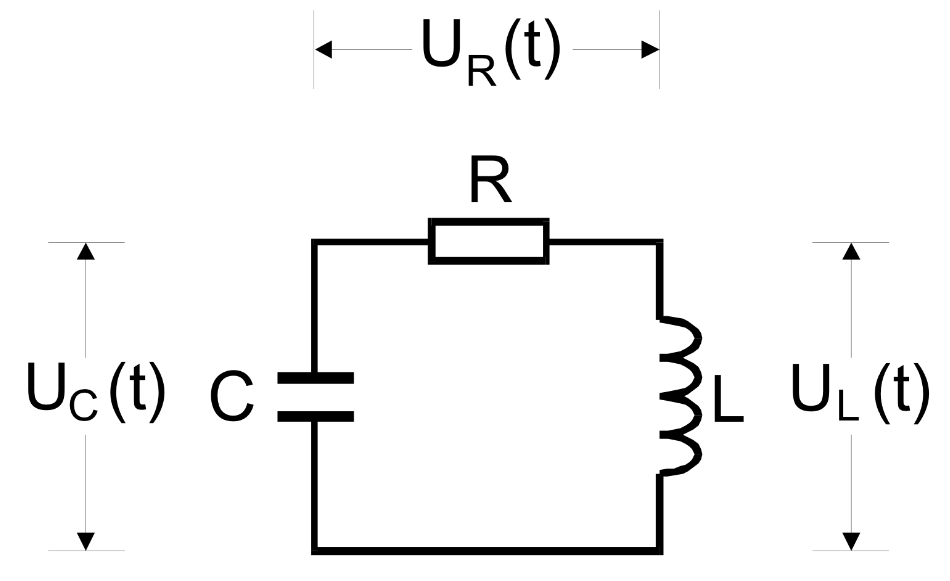
\includegraphics[width=\textwidth]{abb1.jpg}
  \caption{Schematischer Aufbau eines RLC-Kreises\cite{manualV354}}
  \label{fig:abb1}
\end{figure}
Mit Hilfe der 2. Kirchhoffschen Regel lässt sich eine Differntialgleichung zur Beschreibung des Problems finden.
Die in Abbildung \ref{fig:abb1} dargestellten Spannungen addieren sich zu Null:
\begin{equation}
  U_R(t) + U_C(t) + U_L(t)  = 0
  \label{eqn:gl1}
\end{equation}
Die Spannungen können mit dem Ohmschen Gesetz \eqref{eqn:gl2}, dem Induktionsgesetz \eqref{eqn:gl3} und der Defintion der Kapazität \eqref{eqn:gl4} geschrieben werden als:
\begin{equation}
  U_R(t) = RI(t)
  \label{eqn:gl2}
\end{equation}
\begin{equation}
  U_L(t) = L \frac{dI}{dt}
  \label{eqn:gl3}
\end{equation}
\begin{equation}
  U_C(t) = \frac{Q(t)}{C}
  \label{eqn:gl4}
\end{equation}
Daraus folgt die Gleichung:
\begin{equation}
  RI(t) + \frac{Q(t)}{C} + L \frac{dI}{dt} = 0
  \label{eqn:gl5}
\end{equation}
Wird diese nach der Zeit abgeleitet, erhält man die gewünschte Differntialgleichung, die an den harmonischen Oszillator aus der Mechanik erinnert.
\begin{equation}
  \ddot{I}(t) + \frac{R}{L} \dot{I}(t) + \frac{1}{LC}I(t) = 0
  \label{eqn:gl6}
\end{equation}
Ein Lösungsansatz der Gleichung ist:
\begin{equation}
  I(t) = e^{-2\pi\mu t}\left(\symbfcal{A}_1 e^{\text{i}2\pi\nu t} + \symbfcal{A}_2 e^{-\text{i}2\pi\nu t}\right)
  \label{eqn:gl7}
\end{equation}
mit den den komplexen Koeffizienten $\symbfcal{A}_1$ und $\symbfcal{A}_2$ und den Abkürzungen:
\begin{equation}
  \mu := \frac{R}{4\pi L}
  \label{eqn:gl8}
\end{equation}
\begin{equation}
  \nu := \frac{1}{2\pi} \sqrt{\frac{1}{LC} - \frac{R^2}{4L^2}}
  \label{eqn:gl9}
\end{equation}
Die Form der Lösung ist im Besonderen von $\nu$ abhängig, das je nachdem ob die Diskriminante positiv oder negativ ist, reel oder komplex wird.
Deshalb wird für die weitere Betrachtung eine Fallunterscheidung vorgenommen.
\begin{description}
  \item[1. Fall:] $\nu$ ist reel, $\frac{1}{LC} > \frac{R^2}{4L^2}$
\end{description}
Wird für die Koeffizienten der Ansatz
\begin{equation*}
  \symbfcal{A}_1 = \frac{1}{2} A_0 e^{\text{i}\phi} \text{ und } \symbfcal{A}_2 = \frac{1}{2} A_0 e^{-\text{i}\phi}
\end{equation*}
gewählt, lässt sich Gleichung \eqref{eqn:gl7} schreiben als:
\begin{equation}
  I(t) = e^{-2\pi\mu t}\left(A_0 \frac{e^{\text{i}(2\pi\nu t + \phi)} + e^{-\text{i}(2\pi\nu t + \phi)}}{2}\right)
  \label{eqn:gl10}
\end{equation}
Unter Berücksichtigung der Eulerschen Formel lässt sich diese Gleichung weiter umformen zu:
\begin{equation}
  I(t) = A_0 e^{-2\pi\mu t}\cos(2\pi\nu t + \phi)
  \label{eqn:gl11}
\end{equation}
Wie zu erkennen ist nimmt die Amplitude der Cosinus-Funktion exponentiell ab, der RLC-Kreis durchläuft also eine gedämpfte Schwingung (siehe Abbildung \ref{fig:abb2}).
\begin{figure}
  \centering
  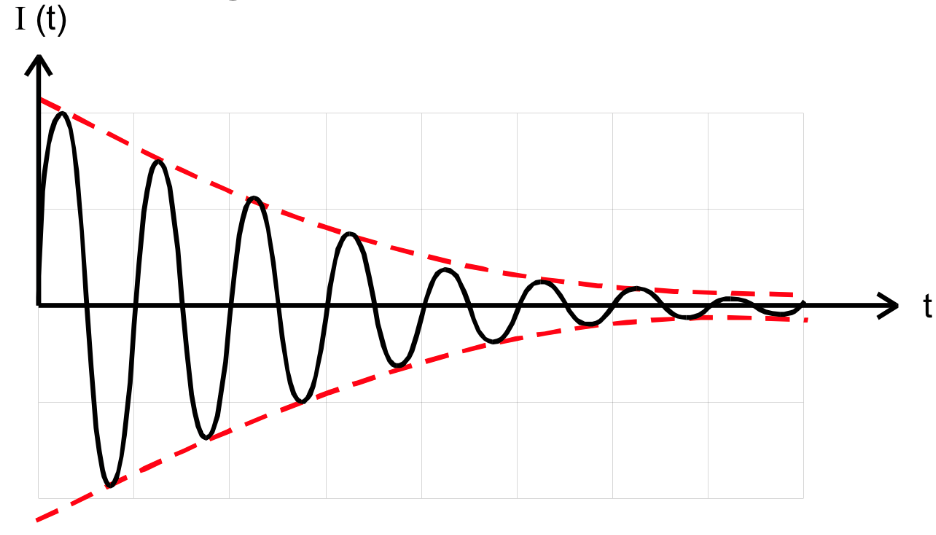
\includegraphics[width=\textwidth]{abb2.jpg}
  \caption{Darstellung einer gedämpften Schwingung\cite{manualV354}}
  \label{fig:abb2}
\end{figure}
Für diese ist die Abklingzeit definiert mit:
\begin{equation}
  T_{ex} := \frac{1}{2\pi\mu} = \frac{2L}{R}
  \label{eqn:gl12}
\end{equation}
\begin{description}
  \item[2. Fall:] $\nu$ ist imaginär, $\frac{1}{LC} < \frac{R^2}{4L^2}$
\end{description}
Wenn $\nu$ imaginär ist, werden alle Exponenten von Gleichung \eqref{eqn:gl7} reel und damit findet keine Schwingung mehr statt.
Dieser Fall wird aperiodische Dämpfung genannt (siehe Abbildung \ref{fig:abb3}).
\begin{figure}
  \centering
  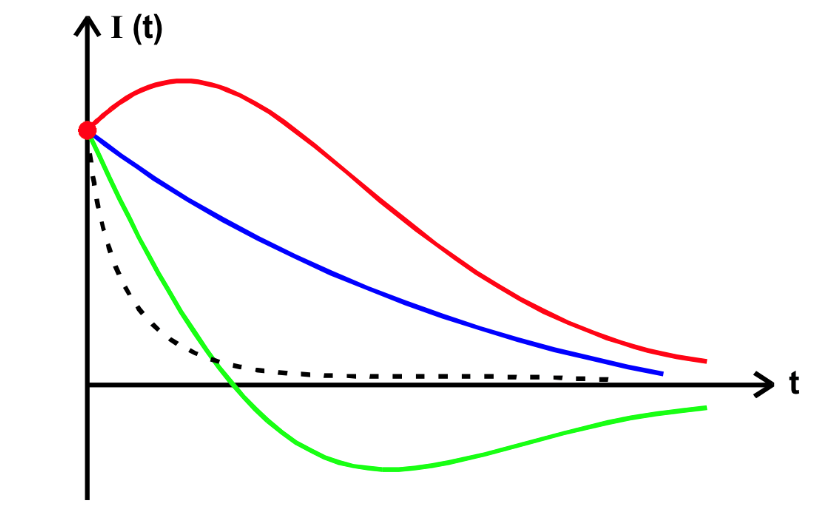
\includegraphics[width=\textwidth]{abb3.jpg}
  \caption{aperiodische Dämpfung und aperiodischer Grenzfall\cite{manualV354}}
  \label{fig:abb3}
\end{figure}
Durch die Wahl von $\symbfcal{A}_1$ und $\symbfcal{A}_2$ wird bestimmt, ob der Lösungsansatz \eqref{eqn:gl7} einen oder keinen Exxtremwert besitzt.
Die Stromstärke $I(t)$ fällt exponentiell und es gilt die proportionale Beziehung:
\begin{equation}
  I(t) \propto \exp\left(\middle[-\frac{R}{2L} \pm \sqrt{\frac{R^2}{4L^2} - \frac{1}{LC}}\middle]t\right)
  \label{eqn:gl13}
\end{equation}
\begin{description}
  \item[3. Fall:] aperiodischer Grenzfall, $\frac{1}{LC} = \frac{R_{ap}^2}{4L^2}$
\end{description}
Unter dieser Bedingung ist $\nu = 0$ und Gleichung \eqref{eqn:gl7} vereinnfacht sich zu:
\begin{equation}
  I(t) = A_0 e^{-2\pi\mu t}
  \label{eqn:gl14}
\end{equation}
Die Stromstärke $I(t)$ fällt hier am schnellsten gegen Null ab ohne dabei überzuschwingen (siehe Abbildung \ref{fig:abb3}).

\subsection{getriebner Schwingkreis}
\label{sec:getrieben}
Der elektische Schwingkreis kann durch eine externe Spannungsquelle getrieben, die periodisch Energie in den Kreis pumpt (siehe Abbildung \ref{fig:abb4}).
\begin{figure}
  \centering
  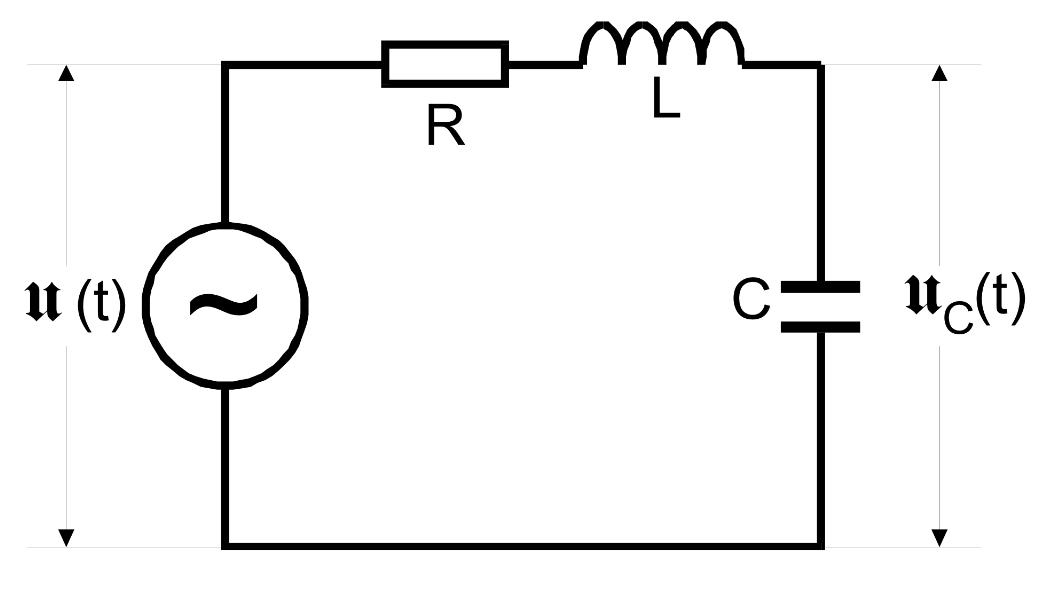
\includegraphics[width=\textwidth]{abb4.jpg}
  \caption{Darstellung eines getriebenen Schwingkreises\cite{manualV354}}
  \label{fig:abb4}
\end{figure}
Das führt zu einer erzwungenen Schwingung mit der Frequenz der Wechselstromquelle.
Diese äußere Anregung kann in der Differntialgleichung \eqref{eqn:gl5} berücksichtig werden, indem diese um eine Inhomogenität ergänzt wird.
$I(t)$ und dessen zeitliche Ableitungen werden unter Ausnutzung von \eqref{eqn:gl4} durch die Kondensatorspannung $U_C$ ersetzt.
\begin{equation}
  LC\ddot{U}_C(t) + RC\dot{U}_C(t) + U_C(t) = U_0e^{\text{i}\omega t}
  \label{eqn:gl15}
\end{equation}
Das Problem wird gelöst für den Ansatz:
\begin{equation}
  U_C(\omega,t) = U(\omega)e^{\text{i}\omega t}
  \label{eqn:gl16}
\end{equation}
Für die Amplitude $U(\omega)$ ergibt sich dann:
\begin{equation}
  U(\omega) = \frac{U_0(1 - LC \omega^2 - \text{i}\omega RC)}{(1 - LC\omega^2)^2 + \omega^2 R^2 C^2}
  \label{eqn:gl17}
\end{equation}
Die Phase von $U(\omega)$ entspricht der Phasenverschiebung zwischen Erreger- und Kondensatorspannung:
\begin{equation}
  \phi(\omega) = \arctan\left(\frac{\text{Im}U(\omega)}{\text{Re}U(\omega)}\right) = \arctan\left(\frac{-\omega RC}{1 - LC\omega^2}\right)
  \label{eqn:gl18}
\end{equation}
Nach Gleichung \eqref{eqn:gl16} haben $U(\omega)$ und $U_C(\omega,t)$ den gleichen Betrag, es fogt also:
\begin{equation}
  U_C(\omega,t) = \frac{U_0}{\sqrt{(1 - LC\omega^2)^2 + \omega^2 R^2 C^2}}
  \label{eqn:gl19}
\end{equation}
Die Kondensatorspannung $U_C$ hängt also von $\omega$ ab, für $$ geht $$ und für $$ geht $$.
Bei einer bestimmten Frequenz, der Resonanzfrequenz, wird $U_C$ maximal und kann größer als $U_0$ werden.
\begin{equation}
  \omega_{\text{res}} = \sqrt{\frac{1}{LC} - \frac{R^2}{2L^2}}
  \label{eqn:gl20}
\end{equation}
Von besonderer Interesse ist das Resonanzphänomen bei schwacher Dämpfung.
\begin{equation*}
  \frac{R^2}{2L^2} << \frac{1}{LC}
\end{equation*}
Unter dieser Bedingung nähert sich die Resonanzfrequenz der Eigenfrequenz des Systems, die definiert ist als:
\begin{equation}
  \omega_0 = \sqrt{\frac{1}{LC}}
  \label{eqn:gl21}
\end{equation}
Der Zusammenhang zwischen $U(\omega)$ und $U_C(\omega,t)$ (siehe Gleichung \eqref{eqn:gl16}) vereinfacht sich zu
\begin{equation}
  U_{C,\text{max}} = \frac{1}{\omega_0 RC}U_0 = qU_0,
  \label{eqn:gl22}
\end{equation}
wobei $q$ als Güte bezeichnet wird.
Ein weiteres Merkmal der Resonanz ist die Breite der Resonanzkurve, die durch die Frequenzen, $\omega_+$ und $\omega_-$ bestimmt ist, bei denen $U_C$ auf $\frac{U_{c,\text{max}}}{\sqrt{2}}$ abgefallen ist.
Daraus lassen sich folgende Beziehungen ableiten:
\begin{equation}
  q = \frac{\omega_0}{\omega_+ - \omega_-}
  \label{eqn:gl23}
\end{equation}
\begin{equation}
  \omega_+ - \omega_- \approx \frac{R}{L}
  \label{eqn:gl24}
\end{equation}
